%&pdflatex
\documentclass[11pt]{article}

\usepackage{geometry}                % See geometry.pdf to learn the layout options. There are lots.
\usepackage{listings}
\usepackage{graphicx}
\usepackage{hyperref}
\usepackage{bookmark}
\geometry{letterpaper}                   % ... or a4paper or a5paper or ...


\setlength{\parindent}{0pt}
\setlength{\parskip}{\baselineskip}%

\title{Programming Applications (PRA) \\ Minor Coursework Exercise 2 \\
``There's a starman waiting in the GUI'' (2.5\%)}
%\author{Martin Chapman (martin.chapman@kcl.ac.uk)}
\date{}                                           % Activate to display a given date or no date

\begin{document}
\maketitle
%\section{}
%\subsection{}

\vspace{-10mm}

\textbf{Please read the document marked `Q\&A Lab Projects and Pair Programming' carefully, before attempting any lab project. It contains important information on how to complete each minor piece of coursework. You will be asked to officially declare that you have read this document prior to submission. False declarations are taken seriously by both the department and by the college.}

\emph{This lab project counts for 2.5\% of your mark for PRA minor coursework assessment, and is the second of four.}

\emph{The release weeks for this assignment start 6th February, at 23:55, and end 20th February, at 23:55. All submissions must occur before the end of the second release week.}

\emph{If you have any questions about the structure of this assessment, please follow the `Additional Support' steps listed on KEATS.}

\textbf{You must select and work with a new partner for this piece of work.}

The aims of the second lab project are as follows:

\begin{enumerate}
	
	\item To explore the roles different widgets can have in a GUI;
	\item To continue the exploration of GUI layouts that began in your first Code Dojo;
	\item To employ simple event handlers and to understand the implications of Swing concurrency;
	\item To understand how to layout and structure GUI code;
	\item To solve basic problems in Java.

\end{enumerate}

\section{Domain Description}

Last weekend, I watched an excellent film called `The Martian' starring Matthew Damon, and now I'm going to ask you to complete a piece of coursework based upon a scene from it. 

In this film, Matthew is stuck on Mars. He has no way of communicating with Earth, until he digs up the Mars Pathfinder, an old rover that NASA lost contact with back in 1997.  

In the scene in question, Matthew discovers that he can use the rover's (still functioning) camera to establish a crude form of two-way communication with NASA back on Earth. Naturally, Matthew can write on a white board and show this to the camera to speak to NASA, but NASA can only communication back by using the camera, and its ability to turn 360 degrees horizontally, as a crude form of \emph{pointing} device. So, with three signs placed into the ground on Mars (one question in the centre, and two answers to the left and to the right, as shown in Figure \ref{fig:signs} below),  NASA can remotely point the camera to a sign, and Matthew can check to see which sign the camera is being pointed at in order to obtain a response to some basic questions.

\begin{figure}[htbp]
\begin{center}
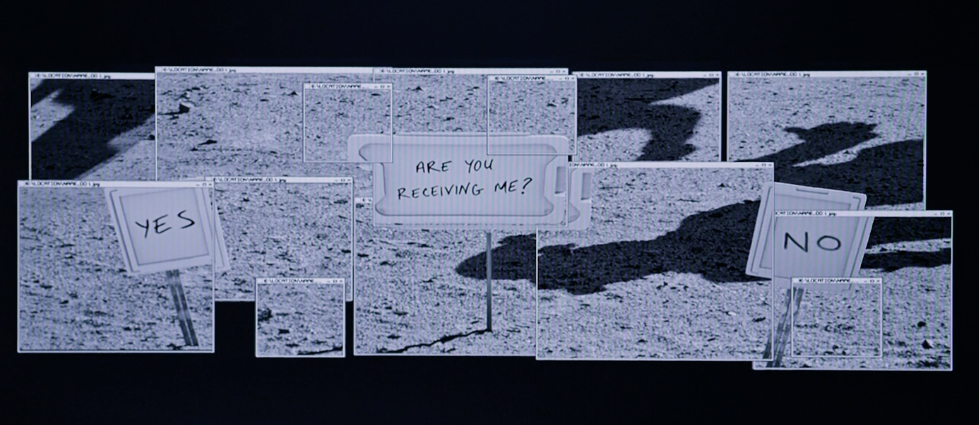
\includegraphics[width=350pt,height=200pt]{/Library/Server/Web/Data/Sites/webserver/PRA/distribute/CSnUsTh4/Assignment2Images/signs.jpg}
\caption{The signs used by Matthew to elicit a response to the question `Are you receiving me?'. Upon observing this image, NASA should either move the camera left to point to a response of `Yes' to the question posed, or to the right to point to a response of `No' to the question posed. Note that a response of `No' would not make sense in this context.}
\label{fig:signs}
\end{center}
\end{figure}


However, as pointed out in the film, this method does not scale well to prolonged  communication. Moreover, the natural extension to this system, in which 26 signs (for each letter of the alphabet) are positioned around the camera in a circle and then pointed to in turn in order to spell out words, is not viable, given that with only 360 degrees of rotation available, it becomes difficult to determine the marginal difference in rotation between adjacent letters.

Being the smart man that he is, Matthew realises that he actually only needs 16 signs placed around the rover in order to facilitate full conversation. This is because the character encoding system ASCII maps every letter of the alphabet to an 8-bit binary number, which can in turn (as you know from 4CCS1CS1) be easily translated into a \emph{pair} of hexadecimal numbers. Therefore, only 16 signs are needed because the hexadecimal system only consists of 16 unique characters (0 - 9 and A - F). After informing NASA to communicate with him using hexadecimal ASCII encoding, Matthew can place his 16 signs around the rover and then note down a series of  characters pointed to in turn by the rover's camera. He can then translate this series back to the full Latin alphabet using an ASCII \emph{table}, remembering that two hexadecimal characters stand for a single Latin character. Thus, communication is established.

A comprehensive recreation of this process is shown here

\begin{quote}
\url{http://www.dcs.kcl.ac.uk/staff/martin/matthewdamon/}
\end{quote}

with the initial question and answer system shown up until 00:52, and the ASCII encoding process shown between 00:52 to 2:47. From 2:47 onwards, things get a little abstract.

In this lab project, we're going to create a program that accepts a series of words written in the Latin alphabet (entered by NASA on Earth, we might imagine), translates them into hexadecimal (via ASCII encoding) and then outputs them to a graphical representation of the rover's pointing camera mechanism. 

\section{Setting up the package}

Create a new \emph{project} in your chosen IDE. Inside this project, create a new \emph{package} named according to a concatenation of your first name, and the first name of your partner ($<$partnerApartnerB$>$). So, if Martin Chapman and Steffen Zschaler were embarking on this exercise, our project would contain a package called \emph{steffenmartin}. The order of names here is unimportant, but it is essential that you name your top-level package in this way, in order to identify your association with your partner to us.

If you locate the actual \emph{folder structure} created in your filesystem by your IDE for this project, you should now find an empty $<$\emph{partnerApartnerB}$>$ folder inside the source folder for your project. 

\section{Creating the Rover's Camera Movement}
\label{section:camera}

In order to represent the rover's camera movement, and the signs it points to, we're going to, rather unimaginatively, use a slider. We will imagine that each point on the slider, and its associated label, represents one of the signs pushed into the ground around the rover. So, to translate the simple signs reading `yes' and `no' in Figure \ref{fig:signs} into a Java GUI, we would produce the following slider (Figure \ref{fig:slider}):

\begin{figure}[htbp]
\begin{center}
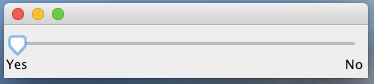
\includegraphics[width=300pt,height=70pt]{/Library/Server/Web/Data/Sites/webserver/PRA/distribute/CSnUsTh4/Assignment2Images/slider.jpg}
\caption{Note that this is an exemplar slider, and does not need to be replicated in your own GUI.}
\label{fig:slider}
\end{center}
\end{figure}

The value currently selected by the slider represents the sign at which the camera is currently pointing, and sliding from one point to another represents the camera moving from pointing to one sign to pointing to another. In the Figure \ref{fig:slider} therefore, we would say the camera is pointing to `Yes'. In order to point to 16 different signs, our slider will, instead, need 16 points (0 - 15) and labels (0 - 9 and A - F). The fact that, in the real world, these signs would be positioned around the rover in a circle (as shown in the video above), as opposed to a straight line, is a point that we will ignore via \emph{abstraction}. 

Whether the rover's \texttt{Camera} enters an \emph{is-a} or a \emph{has-a} relationship with a slider component in order to model the position of the camera is up to you. Both have benefits and drawbacks. Regardless of which you choose, ensure your \texttt{Camera} gives the slider an appropriate size, and configures the slider so that it shows the 16 labels described above. This will also require you to manipulate the lower and upper bounds of the slider in accordance with the number of labels. Assume the slider always starts at 0.

\texttt{Camera} should also have the ability to accept a series of integer positions, which are used, in turn, to set the value of the slider. Conceptually, this allows us to represent a sequence of rotations made by the camera in order to point to different signs (this contrasts the manual left and right movements made using the camera in the video provided). So, when passed the list \texttt{\{1, 5, 12\}}, \texttt{Camera} should adjust the slider to first be at label `1', then at label `5', and then at label `C'; the camera moves to point at 1, then 5 and the C, in sequence. Note that each alphabetic label has an associated numeric position on the slider (e.g. A = 10, B = 11 etc.). Once the slider has been moved to the last label in the list, the process stops, and the slider remains on this label.

You should use \texttt{Thread.sleep(N)} to control the pace at which the content in the slider is set, where the value \texttt{N} dictates this speed. 

\section{Creating NASA's input}

To model input sent to the rover's camera, by NASA in this domain, we are going to create a text input box, the content of which, upon the press of a button, will be translated to hexadecimal, and sent to the camera (the slider) as a sequence of integers in order to move it.

To do this, you should have a \texttt{Communication} frame that will display all the entities involved in the communication. Give this frame an appropriate title (I will refer to this as the default title). For your own sanity, you should also add a call to the method \texttt{setDefaultCloseOperation} (part of the \texttt{JFrame} class) somewhere in your \texttt{Communication} class, with the parameter \texttt{JFrame.EXIT\_ON\_CLOSE}. This will kill the frame application when you close the frame, as opposed to just hiding it, and avoid a build up of open applications. 

To the top of the frame, you should add your \texttt{Camera}. To the bottom of the frame you should add a button with the text `Send'. In the middle of the frame you should add a text area. When you change the size of the frame, the slider associated with your \texttt{Camera} should stay at the top of the frame (but expand to fill any increase in horizontal space) and the send button should stay at the bottom of the frame (but expand to fill any increase in horizontal space). The text area should expand to fill any additional space, both horizontally and vertically. A mockup of this frame is shown below in Figure \ref{fig:mockup}.

\begin{figure}[htbp]
\begin{center}
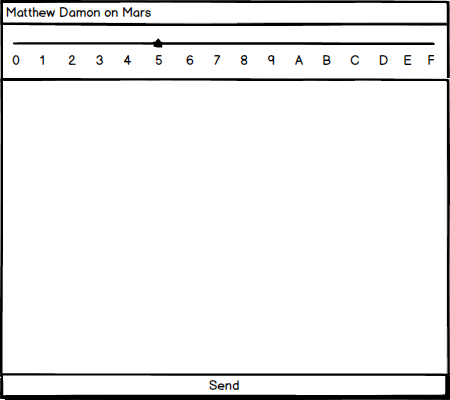
\includegraphics[width=210pt,height=180pt]{/Library/Server/Web/Data/Sites/webserver/PRA/distribute/CSnUsTh4/Assignment2Images/mockup.png}
\caption{Mockup of required GUI.}
\label{fig:mockup}
\end{center}
\end{figure}

To translate the text entered into the text area into hexadecimal, I have provided an ASCII table (\texttt{ascii\_table.csv}) on KEATS. You should download this, and read it into your program at an appropriate point in order to build up a programmatic version of the table. So, when the user presses `Send', each character from the text area should be passed to this table and the \textbf{two character} hexadecimal equivalent should be recorded.

You must \textbf{not} employ any existing functions to change your letters into hexadecimal (e.g. \texttt{toString(16)}) as this will result in you losing marks. 

Once each character from the text area has been translated into its two character hexadecimal equivalent, each \emph{individual} hexadecimal character must be translated into an integer, so that it can be passed, within a list, to the camera in order to specify a sequence of rotations towards different signs, as discussed in Section \ref{section:camera}. Because the camera only accepts a list of integers (in order to set the value of the slider), hexadecimal values between A and F must be converted to their integer equivalents (e.g. A to 10, B to 11, etc.).

You must \textbf{not} employ any existing functions to change your letters from hexadecimal to integer values (e.g. \texttt{parseInt(hexValue, 16)}) as this will result in you losing marks. 

Once you have a list of integers, derived from translating each character from the text area into its two character hexadecimal equivalent, and then translating any alphabetic (non-integer) hexadecimal character into their integer form, pass this list to the camera. As a result, pressing the `Send' button should start the slider moving.

Table \ref{table:process} summarises the required conversion processes when the `Send' button is clicked:

\begin{table}[h!]

	\begin{center}

		\begin{tabular}{p{8cm}p{6cm}}
			\hline
			Action & Input \\
			\hline
			Enter Latin text into the text area & ``DAMON'' \\
			\hline
			Convert this text to hexadecimal using the ASCII table & `D' = 44, `A' = 41, `M' = 4D, `O' = 4F, `N' = 4E \\
			\hline
			Convert any alphabetic characters into their numeric equivalent & `D' = 44, `A' = 41, `M' = 4,13, `O' = 4,15, `N' = 4,14 \\
			\hline
			Pass this as a string of integer to \texttt{Camera} in order to dictate movement points & \texttt{\{4, 4, 4, 1, 4, 13, 4, 15, 4, 14\}} \\
			\hline
			Slider moves to 4, then stays on 4, then stays on 4, then moves to 1, then to 4, and then to D, etc. & - \\
			\hline
		\end{tabular}
		
		\caption{The process of converting from a String to a sequence of slider movements.}
		\label{table:process}

	\end{center}

\end{table}%

Once the `Send' button has been pressed, the title of the \texttt{Communication} frame should change from the default title to `Sending...', and should remain as such until the slider stops moving. Once the movement is over, the title of the frame should change back to the default title, to indicate that the slider's movement has ended.

\subsection{Swing and Concurrency}

When implementing the functionality for your  `Send' button, you will be referencing code (inside \texttt{Camera}) that iteratively updates the state of another component (your slider). Because all Swing operations are executed on the same \emph{thread}, they are always performed sequentially. However, in this case, we want two Swing operations to execute \emph{simultaneously}: the button event, and the update to the slider. Without alteration therefore, our code will not operate in the way that we want. Instead, while the update to the slider's value (and the associated thread sleep) will execute as normal, the effect of these updates will not be \emph{visible} until \emph{after} the button press event. The button press event ends after all the iterative updates to the slider (i.e. when all of its prescribed functionality is complete), at which point the state of the slider will be the last integer value passed. So, unless you have already anticipated this issue, after pressing the `Send' button, rather than seeing a sequence of moves made by the slider, after a delay, the slider will simply jump to the last integer in the passed list.

You can read more about concurrency in Swing here: \url{http://docs.oracle.com/javase/tutorial/uiswing/concurrency/dispatch.html}.

To mitigate this effect, we must launch a new thread, containing our manipulation of the slider's position, from within the action code associated with the `Send' button. Conduct the appropriate research to learn how to do this, or ask your peers on the KEATS PRA forum (`Your Questions / Our Answers').

\section{Testing your program}

It is essential that you test your program to ensure that the translation process is correct. To do this, you should enter a word into the text area, without your partner observing the word in question, and press `Send'. Then, your partner should note down the hexadecimal characters pointed to by the slider. Once the slider's movement is complete, your partner should translate each pair of hexadecimal characters into a Latin character in order to decode the sent message.

The word you should send to your partner is: _SentWord_. Your partner will also have a word to send to you, so you should repeat this process, except this time you should translate the output of the slider.

To help facilitate this process, you should add an additional action to the code that is executed when the `Send' button is pressed, that removes the message entered into the text area.

Your TA will ask you and your partner to demonstrate this process during your assessment.

\section{Laying everything out}

This task is very simple. Have a look at your code. Chances are, as is often the temptation with Swing code, that you have long sets of lines containing lots of object creation and different method invocations. How could you separate these lines into logical subsets, and put them within different methods? 

Your TA will look for logically separated code during your assessment. 

\section{Model-View-Controller}

Depending on how you have structured your code, there may be structural alterations you can make that better account for the Model-View-Controller design pattern (PRA Lecture 4). You don't need to make any changes to your submission, but think carefully about what these alterations might be. 

Your TA will ask you questions about this during your assessment.

\section{Changing the camera representation (optional)}

As mentioned, using a slider to represent the 360 degrees of movement that a camera might make to face towards a variety of signs is highly unimaginative. Change your implementation so that, rather than showing the position of the camera using a slider, you implement something that is more graphically representative of the camera and the signs, as shown in the video linked to above. Something like the mockup in Figure \ref{fig:mockup-camera}, whereby the arrow moves to indicate the different hexadecimal characters and the view of the rover is from above, would be excellent.

\begin{figure}[htbp]
\begin{center}
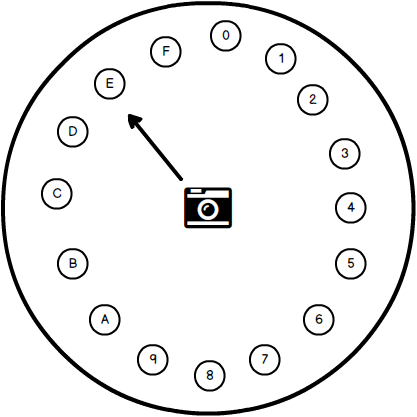
\includegraphics[width=180pt,height=180pt]{/Library/Server/Web/Data/Sites/webserver/PRA/distribute/CSnUsTh4/Assignment2Images/mockup_camera.png}
\caption{A richer graphical representation of the camera and signs used in this domain.}
\label{fig:mockup-camera}
\end{center}
\end{figure}

%Do something with the most imaginative solutions?
Imaginative ideas welcome.

\subsection{Submitting your work}

\textbf{Ensure your code is correctly annotated with Javadoc comments}, in addition to standard comments. This is something we will be expecting to see from now on.

If, once finished, you wish to submit your work to us for preliminary feedback, you should do so by following the `Additional Support' steps from Step 3.2 onwards (i.e. direct contact), in order to avoid sharing your solution with your peers unnecessarily.

If you are happy with your solution, then you should both submit \emph{identical} copies of it to KEATS, adhering to all the submission rules given in the Q\&A document referenced at the beginning of this project brief. Nothing should differ between the submissions, especially the ordering of the names in the top-level package (i.e. $<$\emph{partnerApartnerB}$>$).

The folder you compress for submission should be your top-level package, or the first folder inside your project source. For this assignment, the top-level folder is $<$\emph{partnerApartnerB}$>$. Compress this folder directly, so that the file you submit is of the form $<$\emph{partnerApartnerB}$>$.\\ $<$compression\_extension$>$ (e.g. steffenmartin.zip). The names of the compressed files that you and your partner submit should therefore be identical.

\end{document}
